\documentclass[a4paper,12pt]{article} 

%%% Работа с русским языком
\usepackage{cmap}					% поиск в PDF
\usepackage{mathtext} 				% русские буквы в фомулах
\usepackage[T2A]{fontenc}			% кодировка
\usepackage[utf8]{inputenc}			% кодировка исходного текста
\usepackage[english,russian]{babel}	% локализация и переносы

%%% Дополнительная работа с математикой
\usepackage{amsmath,amsfonts,amssymb,amsthm,mathtools, gensymb} % AMS
\usepackage{icomma} % "Умная" запятая: $0,2$ --- число, $0, 2$ --- перечисление

%%Таблица
\usepackage[table,xcdraw]{xcolor}
\usepackage{caption}
\usepackage{subcaption}
\usepackage{floatrow}
\floatsetup[table]{capposition=top}
\floatsetup[wrapfigure]{capposition=bottom}


%% Номера формул
\mathtoolsset{showonlyrefs=true} % Показывать номера только у тех формул, на которые есть \eqref{} в тексте.

%% Шрифты
\usepackage{euscript}	 % Шрифт Евклид
\usepackage{mathrsfs} % Красивый матшрифт

%% Свои команды
\DeclareMathOperator{\sgn}{\mathop{sgn}}

%% Перенос знаков в формулах (по Львовскому)
\newcommand*{\hm}[1]{#1\nobreak\discretionary{}
{\hbox{$\mathsurround=0pt #1$}}{}}

%% Стиль страницы
\usepackage{fancyhdr}

%% Для рисунков
\usepackage{graphicx}
\usepackage[export]{adjustbox}
\usepackage{float}
\usepackage{ragged2e}
\usepackage{wrapfig}

%Отступы и поля 
\textwidth=20cm
\oddsidemargin=-2cm
\topmargin=-2cm
\textheight=25cm

\pagestyle{fancy}
\begin{document}
\begin{titlepage}
\begin{center}
%\vspace*{1cm}
\large{\small ФЕДЕРАЛЬНОЕ ГОСУДАРСТВЕННОЕ АВТОНОМНОЕ ОБРАЗОВАТЕЛЬНОЕ\\ УЧРЕЖДЕНИЕ ВЫСШЕГО ОБРАЗОВАНИЯ \\ МОСКОВСКИЙ ФИЗИКО-ТЕХНИЧЕСКИЙ ИНСТИТУТ\\ (НАЦИОНАЛЬНЫЙ ИССЛЕДОВАТЕЛЬСКИЙ УНИВЕРСИТЕТ)\\ ФАКУЛЬТЕТ АЭРОКОСМИЧЕСКИХ ТЕХНОЛОГИЙ}
\vfill
\line(1,0){430}\\[1mm]
\huge{Лабораторная 4}\\
\huge\textbf{Статические и динамические библиотеки}\\
\line(1,0){430}\\[1mm]
\vfill
\begin{flushright}
\normalsize{Рогозин Владимир}\\
\normalsize{\textbf{Группа Б03-106}}\\
\end{flushright}
\end{center}
\end{titlepage}
\fancyhead[L] {Лабораторная 4}

\textbf{Пункт 1: Статическая библиотека}

Cтатическая библиотека, по сути, содержит объединённые объектные файлы с инструкциями, которые потом вставляются в бинарный код. Команды подключаются и вставляются в код на этапе линковки. В итоге получаем один исполняемый файл со всеми инструкциями. Очевидным минусом статических библиотек является то, что при обновлении библиотеки придётся перекомпилировать каждый файл, использующий её, а также размер исполняемого файла может сильно увеличиваться при использовании статических библиотек. Создадим простейшую статическую библиотеку, состоящую из одной функции, которая суммирует два целых числа. На первой картинке представлен код программы, использующей эту функцию.
\begin{figure}[H]\label{fig: statCode64}
    \centering
    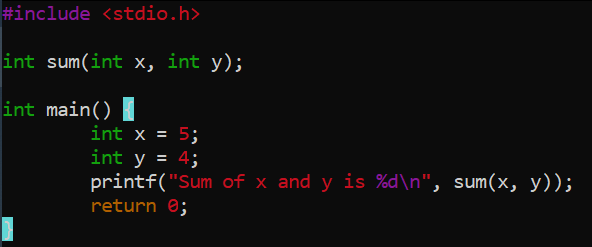
\includegraphics[width = 0.8 \textwidth]{Код использующий стат библиотеку.png}
    \caption{Код программы на С}
\end{figure}

\begin{figure}[H]\label{fig: 32 and 64 func for static library}
    \subfloat[Листинг функции 32-х битной системы]{
    \begin{minipage}[t]{0.5\textwidth}
        \centering
        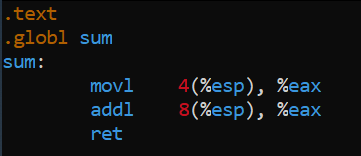
\includegraphics[width = 0.9\textwidth]{Листинг функции С32.png}
    \end{minipage}}
    \subfloat[Листинг функции 64-х битной системы]{
    \begin{minipage}[t]{0.5\textwidth}
        \centering
        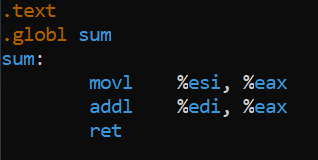
\includegraphics[width = 0.77\textwidth]{Листинг функции С64.png}
    \end{minipage}}
\end{figure}

\begin{figure}[H]\label{fig: statLibCreation}
    \centering
    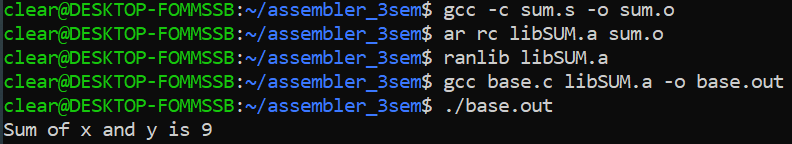
\includegraphics[width = 0.8 \textwidth]{Создание стат библиотеки.png}
    \caption{Создание статической библиотеки}
\end{figure}
Теперь посмотрим на листинг первой программы для обеих систем. Видим, что наша функция \textit{sum} вызывается через \textit{call} с припиской \textit{@PLT} (Procedure Linkage Table), чего бы не было при вызове функции, если бы она была описана в этом же файле. Заметить, что также вызывается и \textit{printf}, то есть можно предположить, что все стандартные функции (\textit{printf, scanf etc.}) реализованы примерно также.

\begin{figure}[H]\label{fig: 32 and 64 static library}
    \subfloat[Листинг программы, использующей функцию sum, 32 бита]{
    \begin{minipage}[t]{0.4\textwidth}
        \centering
        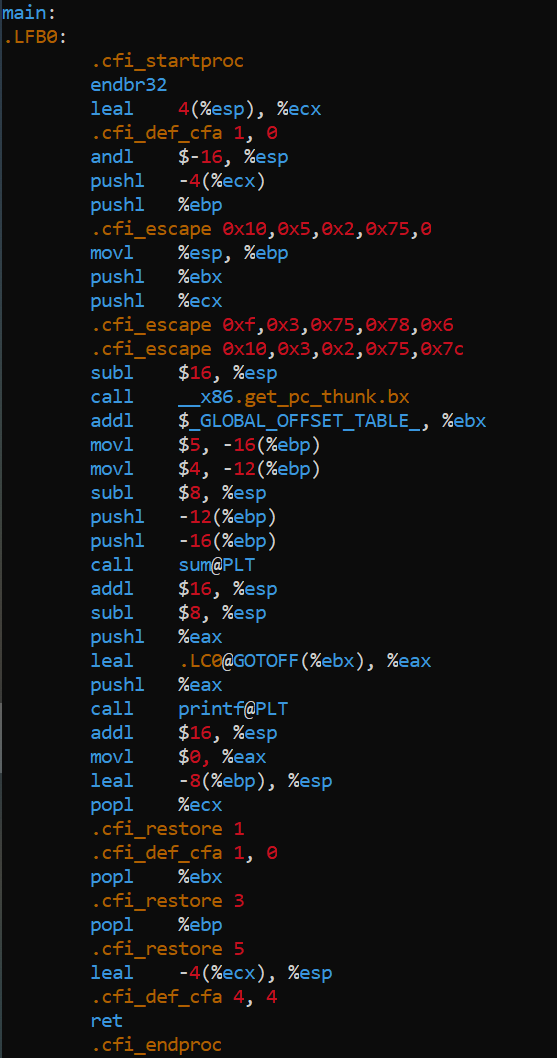
\includegraphics[width = 0.85\textwidth]{Листинг со стат библ 32.png}
    \end{minipage}}
    \subfloat[Листинг программы, использующей функцию sum, 64 бита]{
    \begin{minipage}[t]{0.4\textwidth}
        \centering
        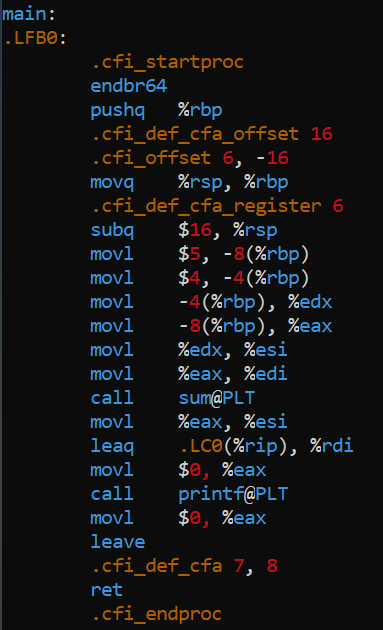
\includegraphics[width = 0.976\textwidth]{Листинг со стат библ 64.png}
    \end{minipage}}
\end{figure}

\textbf{Пункт 2: Динамическая библиотека}

Динамическая библиотека работает немного иначе. Она состоит из подпрограмм, которые подключаются уже во время выполнения. Они не становятся частью бинарника , а так и остаются отдельными модулями, поэтому несколько программ могут использовать одну и ту же копию библиотеки, что может сэкономить много места. Ещё одним преимуществом таких библиотек является возможность легко обновлять файлы(не надо будет перекомпилировать все программы, использовавшие библиотеку до обновления). Минусом использования динамических библиотек может являться сложность в осуществлении связи между библиотекой и программой(система должна знать где и как найти нужную библиотеку). Теперь создадим динамическую библиотеку, посмотрим на листинг программы, использующей функцию из неё.

\begin{figure}[H]\label{fig: dynLibCreation}
    \centering
    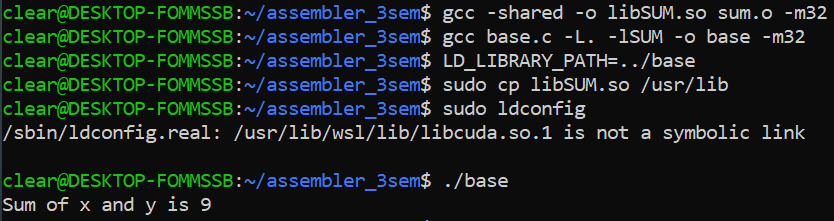
\includegraphics[width = 0.8 \textwidth]{Создание дин библиотеки.png}
    \caption{Создание динамической библиотеки}
\end{figure}

Команда \textit{ldconfig} создаёт необходимые привязки для динамических библиотек, которые используются компановщиками, которые выполняют связывание во время выполнения. \textit{LD\_LIBRARY\_PATH} указывает где следует искать библиотеку.    

Ассемблерные листинги абсолютно идентичны тем, которые получились в первом пункте. Функция $sum$ вызывается точно также.

\begin{figure}[H]\label{fig: 32 and 64 dynamic library}
    \subfloat[Листинг программы, использующей функцию sum, 32 бита]{
    \begin{minipage}[t]{0.4\textwidth}
        \centering
        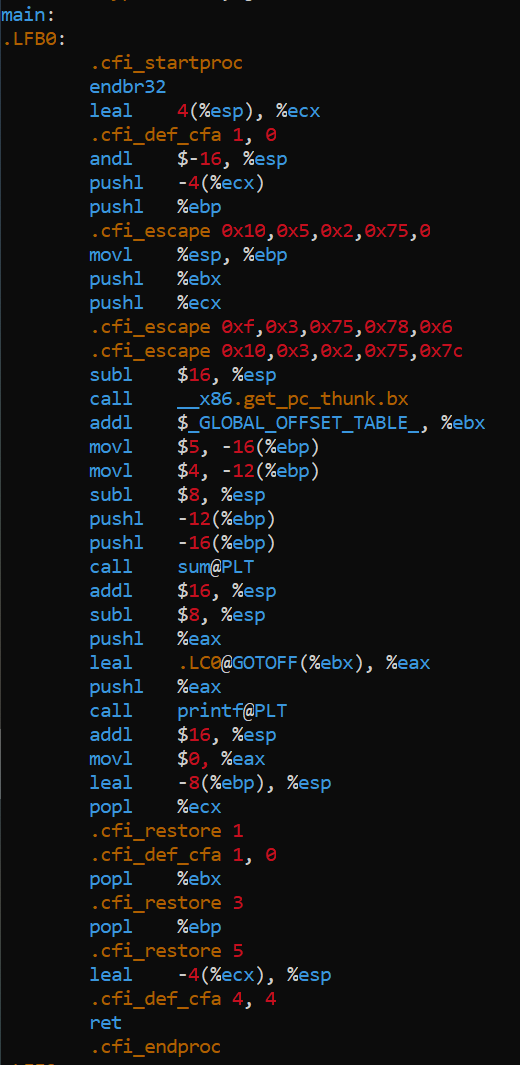
\includegraphics[width = 0.82\textwidth]{Листинг с дин библ 32.png}
    \end{minipage}}
    \subfloat[Листинг программы, использующей функцию sum, 64 бита]{
    \begin{minipage}[t]{0.4\textwidth}
        \centering
        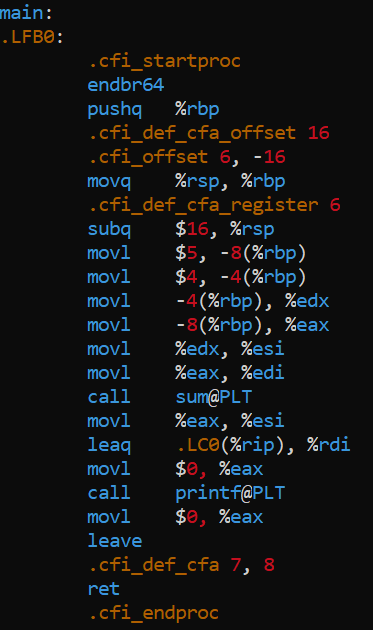
\includegraphics[width = 0.996\textwidth]{Листинг с дин библ 64.png}
    \end{minipage}}
\end{figure}

\newpage
\textbf{Пункт 3: Смотрим на бинарники}

С помощью \textit{objdump} посмотрим на бинарники в обоих случаях. Видим различия в местах вызова функции: в случае статической библиотеки идёт переход на строчку, где описана функция, в случае динамической библиотеки программа переходит на строчку, где лежат инструкции о том, где искать сам исполняемый файл. Заметны различия и в номерах строк куда переходит программа. В первом случае функция описана под \textit{main'}ом(номер 117с, \textit{main} заканчивается на 117b), во втором случае гораздо дальше, но примерно там же и лежит \textit{printf}(номера 1070 и 1060 соответственно).      
\begin{figure}[H]\label{fig: bin stat}
    \centering
    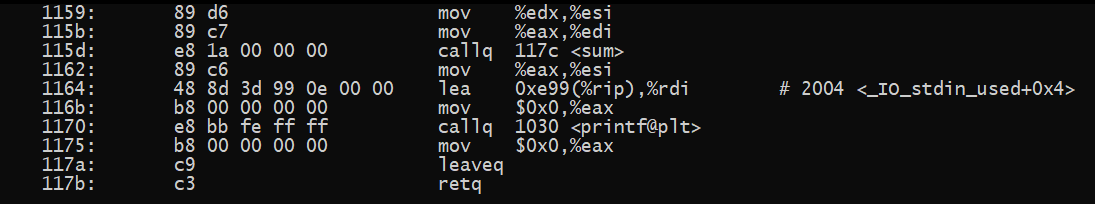
\includegraphics[width = \textwidth]{Бинарник стат библ.png}
    \caption{Бинарник программы, использующей статическую библиотеку}
\end{figure}

\begin{figure}[H]\label{fig: bin dyn}
    \centering
    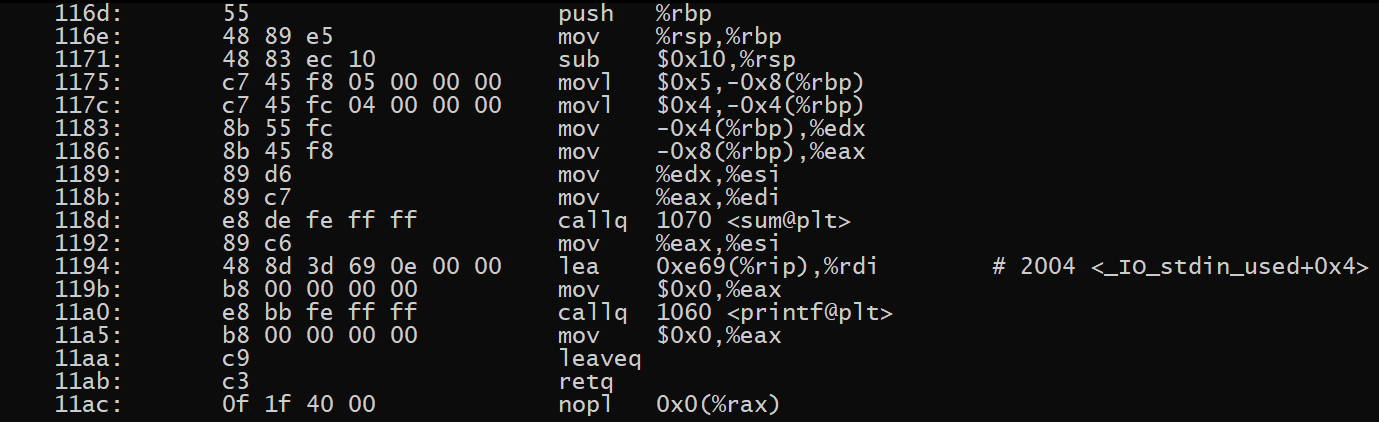
\includegraphics[width = \textwidth]{Бинарник дин библ.png}
    \caption{Бинарник программы, использующей динамическую библиотеку}
\end{figure}

\end{document}
